\documentclass[]{article}

\usepackage{tikz}
\usepackage{lipsum}  % For generating dummy text

\usetikzlibrary {intersections}

%opening
\title{}
\author{}

\begin{document}

\maketitle

\begin{abstract}
See :

https://whitneyberard.com/tikzexamples.pdf

% Also - https://www.overleaf.com/learn/latex/LaTeX_Graphics_using_TikZ%3A_A_Tutorial_for_Beginners_(Part_1)%E2%80%94Basic_Drawing
% https://tikz.dev/tutorial


\end{abstract}

\section{Diagram Examples}

\subsection{Rectangle - 01}

\begin{tikzpicture}
	\draw (0,0) -- (4,0) -- (4,4) -- (0,4) -- cycle;
\end{tikzpicture}

\subsection{Rectangle - 02}

\begin{tikzpicture}
	\draw (0,0) rectangle  (4,4);
\end{tikzpicture}

\newpage



\subsection{Drawing Parabolas}

Draw a parabola -> (vertex) parabola (point)

xxx

\begin{tikzpicture}
	\draw (4,0) parabola  (1,4);
\end{tikzpicture}

xxx

\begin{tikzpicture}
	\draw[thick] (-1,-2) parabola bend (1,2) (3,-2);
\end{tikzpicture}


\begin{tikzpicture}
\draw[thick] (0,3) parabola (2,0);
\draw[thick] (4,-3) parabola (2,0);
\draw[thick] (4,-3) parabola (6,0);
\draw[thick] (7,2) parabola (6,0);
\end{tikzpicture}

\begin{tikzpicture}
\draw[thick] plot[smooth, tension=.7] coordinates {(-1.5,3) (0,-1) (3,2.5) (5,-3)};
\end{tikzpicture}


\begin{tikzpicture}
	\draw (4,0) parabola  (-4,4) |- (1,0);
\end{tikzpicture}

\begin{tikzpicture}
	\draw (0,0) parabola (1.5,2.25) ;
	\draw (0,0) parabola (-1.5,2.25) ;
\end{tikzpicture}


\subsection{Rectangle}

\begin{tikzpicture}
	\draw (0,0) .. controls (0,4) and (4,0) .. (4,4);
\end{tikzpicture}

\subsection{Circle}

\begin{tikzpicture}
	\draw (0,0) circle  (3cm);
\end{tikzpicture}

\subsection{Ellipse}

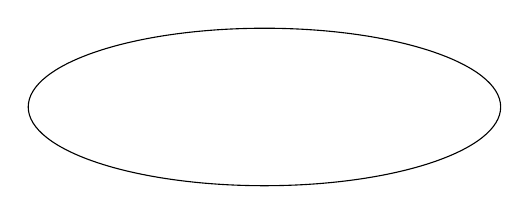
\begin{tikzpicture}
	\draw (0,0) ellipse  (3cm and 1cm);
\end{tikzpicture}

\subsection{Arc}

\begin{tikzpicture}
	\draw (0,0) arc  (0:75:3cm);
\end{tikzpicture}

\subsection{Circle}

\begin{tikzpicture}
	\draw[red,thick,dashed]  (2,2) circle  (3cm);
\end{tikzpicture}

\newpage


\subsection{Grids}

\subsubsection{Bounded Grid}


\begin{tikzpicture}
	\draw[step=1cm,gray,very thin]  (-2,-2) grid  (6,6);
\end{tikzpicture}

\subsubsection{Unbounded Grid - Very Thin}

\begin{tikzpicture}
	\draw[step=1cm,gray,very thin]  (-1.9,-1.9) grid  (5.9,5.9);
\end{tikzpicture}

\subsubsection{Unbounded Grid - Thin}

\begin{tikzpicture}
	\draw[step=1cm,gray,thin, dashed]  (-1.9,-1.9) grid  (5.9,5.9);
\end{tikzpicture}

\subsubsection{Unbounded Grid - Thick}


\begin{tikzpicture}
	\draw[step=1cm,blue,thick]  (-1.9,-1.9) grid  (5.9,5.9);
\end{tikzpicture}


\newpage

\section{Graphs as Figures}

\begin{figure}[htbp]
	\centering
	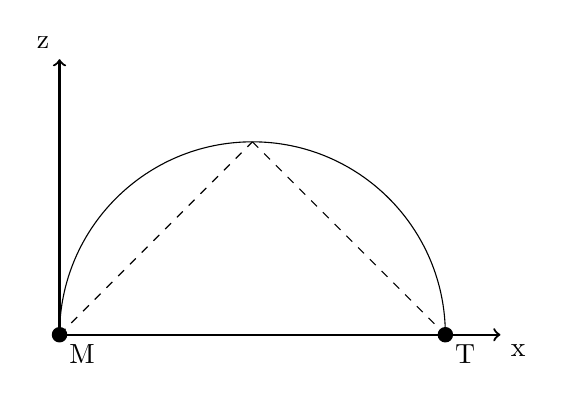
\begin{tikzpicture}[scale = 0.7]
		\draw[thick,->] (0,0) -- (8,0) node[anchor=north west] {x};
		\draw[thick,->] (0,0) -- (0,5) node[anchor=south east] {z};       
		\fill (0,0)  circle[radius=4pt]node[anchor=north west] {M};
		\fill (7,0)  circle[radius=4pt]node[anchor=north west] {T};
		\draw [dashed] (0,0) -- (3.5,3.5);
		\draw [dashed] (3.5,3.5) -- (7,0);
		\draw (7,0) arc (0:180:3.5);
	\end{tikzpicture}
	\caption{}
\end{figure}


\begin{figure}[htbp]
	\centering
	% Note! if you change the scale = 2 to something else in the next line, you need to change the 
	% radius of the circles manually as well.
	\begin{tikzpicture}[scale = 2]
		% Axes
		\draw[->, very thick] (0,0) -- (4.2,0) node[right] {$x$};       % X-axis
		\draw[->, very thick] (0,0) -- (0,3) node[above] {$y$};   % Y-axis
		% The plots
		\draw[scale = 0.5, domain = 0:3, variable = \x, dash pattern = on 3pt off 1.5pt] plot ({\x}, {\x});         % left line
		\draw[scale = 0.5, domain = 3:6, variable = \x, dash pattern = on 3pt off 1.5pt] plot ({\x}, {-\x + 6});    % right line
		\draw[scale =0.15, domain = -4:4, variable = \x]  plot ({\x*3 +12},{-\x*\x + 16});                                  % parabola
		% Labels
		\fill (0,0)  circle[radius=1pt]node[anchor=north west] {M};
		\fill (3,0)  circle[radius=1pt]node[anchor=north west] {T};
		\fill (3.6,0)  circle[radius=1pt]node[anchor=north west] {$\alpha$};
	\end{tikzpicture}
	\caption{}
\end{figure}


\begin{figure}[htbp]
	\centering
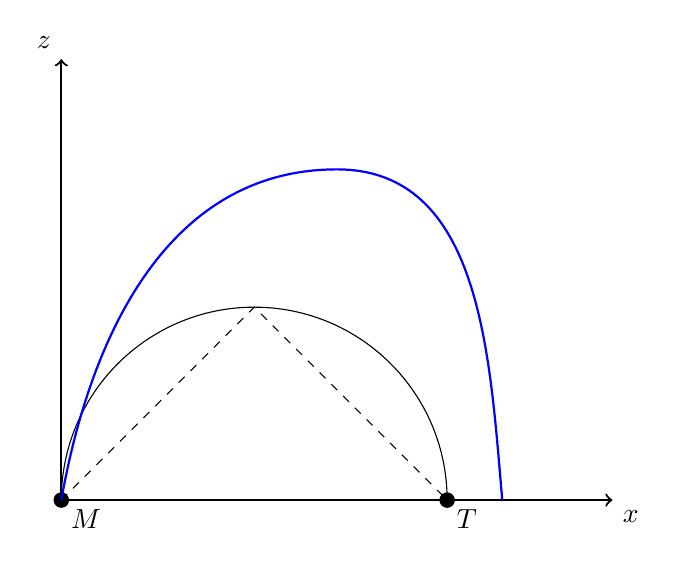
\begin{tikzpicture}[scale = 0.7]
	\draw[thick,->] (0,0) -- (10,0) node[anchor=north west] {$x$};
	\draw[thick,->] (0,0) -- (0,8) node[anchor=south east] {$z$};       
	\fill (0,0)  circle[radius=4pt] node[anchor=north west] {$M$};
	\fill (7,0)  circle[radius=4pt] node[anchor=north west] {$T$};
	\draw [dashed] (0,0) -- (3.5,3.5) -- (7,0);
	\draw (7,0) arc (0:180:3.5);
	\draw[blue,thick] (0,0) to[out=80,in=180] (5,6) to[out=0,in=95] (8,0);
\end{tikzpicture}
	\caption{}
\end{figure}


\newpage

\section{More Complex Graphs}

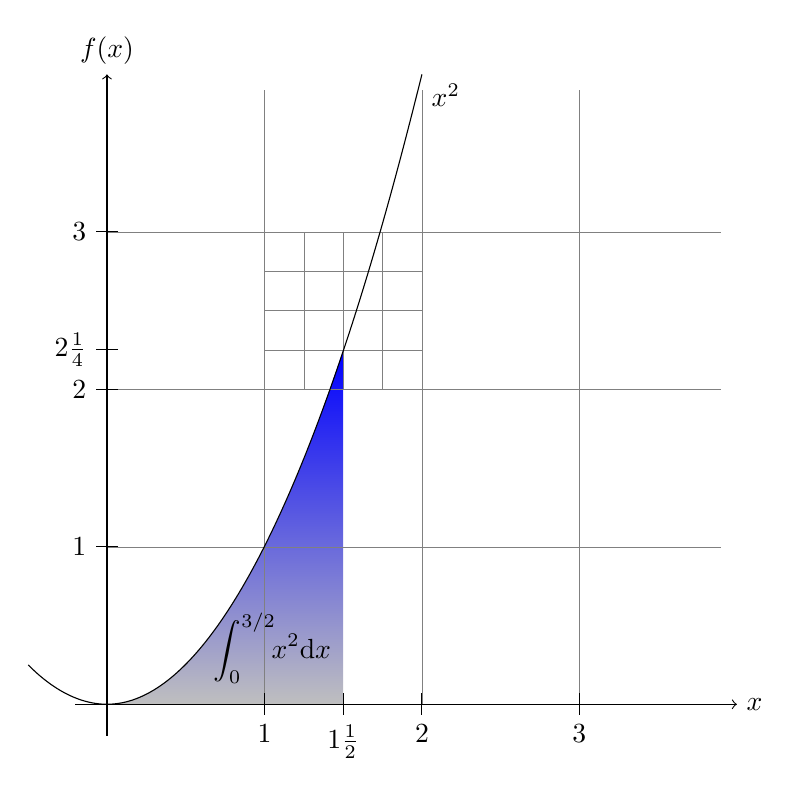
\begin{tikzpicture}[scale=2]
	\shade[top color=blue,bottom color=gray!50] 
	(0,0) parabola (1.5,2.25) |- (0,0);
	\draw (1.05cm,2pt) node[above] 
	{$\displaystyle\int_0^{3/2} \!\!x^2\mathrm{d}x$};
	
	\draw[style=help lines] (0,0) grid (3.9,3.9)
	[step=0.25cm]      (1,2) grid +(1,1);
	
	\draw[->] (-0.2,0) -- (4,0) node[right] {$x$};
	\draw[->] (0,-0.2) -- (0,4) node[above] {$f(x)$};
	
	\foreach \x/\xtext in {1/1, 1.5/1\frac{1}{2}, 2/2, 3/3}
	\draw[shift={(\x,0)}] (0pt,2pt) -- (0pt,-2pt) node[below] {$\xtext$};
	
	\foreach \y/\ytext in {1/1, 2/2, 2.25/2\frac{1}{4}, 3/3}
	\draw[shift={(0,\y)}] (2pt,0pt) -- (-2pt,0pt) node[left] {$\ytext$};
	
	\draw (-.5,.25) parabola bend (0,0) (2,4) node[below right] {$x^2$};
\end{tikzpicture}

\newpage


\section{Complex Circle Graphs}


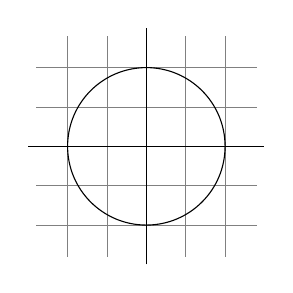
\begin{tikzpicture}
	\draw[step=.5cm,gray,very thin] (-1.4,-1.4) grid (1.4,1.4);
	\draw (-1.5,0) -- (1.5,0);
	\draw (0,-1.5) -- (0,1.5);
	\draw (0,0) circle [radius=1cm];
\end{tikzpicture}

\begin{tikzpicture}[scale=3]
	\draw[step=.5cm,gray,very thin] (-1.4,-1.4) grid (1.4,1.4);
	\draw (-1.5,0) -- (1.5,0);
	\draw (0,-1.5) -- (0,1.5);
	\draw (0,0) circle [radius=1cm];
	\draw (3mm,0mm) arc [start angle=0, end angle=30, radius=3mm];
\end{tikzpicture}

\newpage

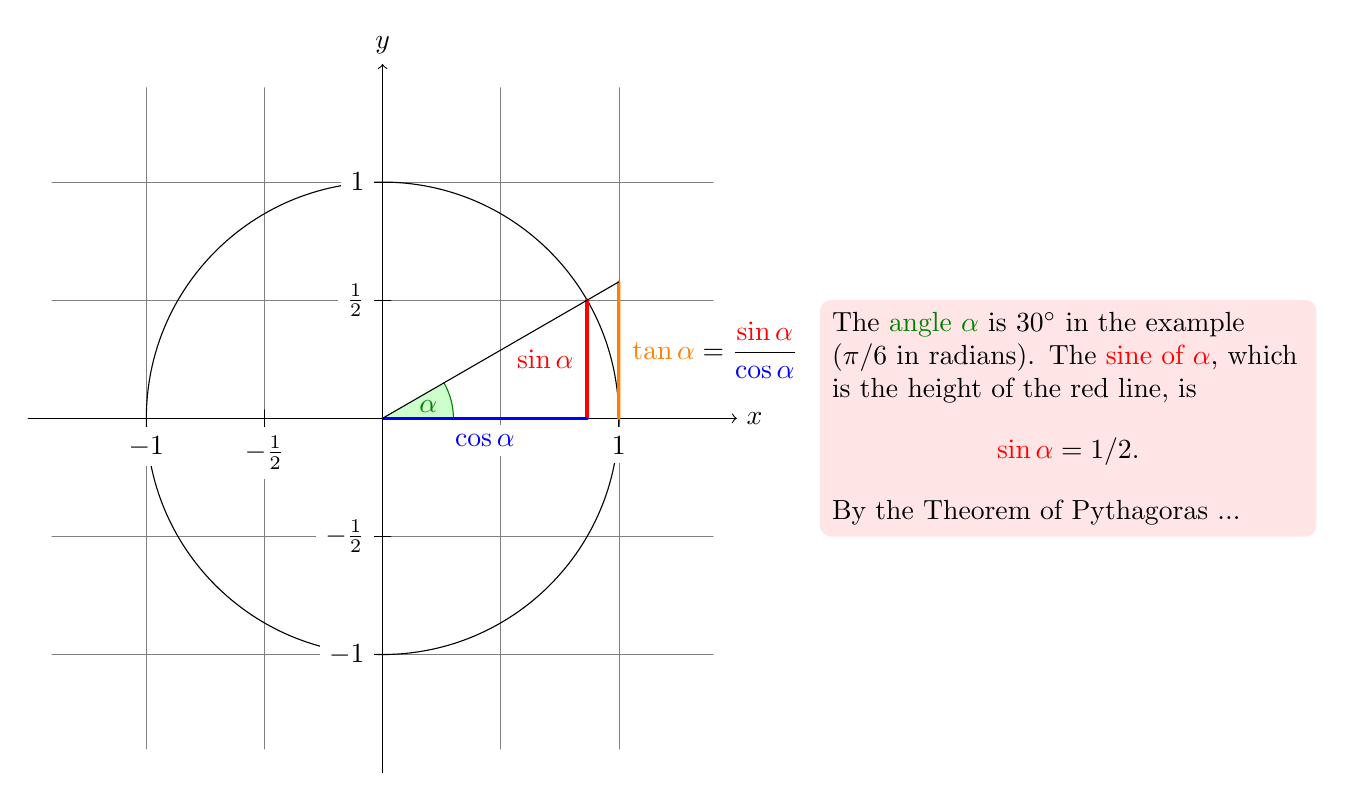
\begin{tikzpicture}
	[scale=3,line cap=round,
	% Styles
	axes/.style=,
	important line/.style={very thick},
	information text/.style={rounded corners,fill=red!10,inner sep=1ex}]
	
	% Colors
	\colorlet{anglecolor}{green!50!black}
	\colorlet{sincolor}{red}
	\colorlet{tancolor}{orange!80!black}
	\colorlet{coscolor}{blue}
	
	% The graphic
	\draw[help lines,step=0.5cm] (-1.4,-1.4) grid (1.4,1.4);
	
	\draw (0,0) circle [radius=1cm];
	
	\begin{scope}[axes]
		\draw[->] (-1.5,0) -- (1.5,0) node[right] {$x$} coordinate(x axis);
		\draw[->] (0,-1.5) -- (0,1.5) node[above] {$y$} coordinate(y axis);
		
		\foreach \x/\xtext in {-1, -.5/-\frac{1}{2}, 1}
		\draw[xshift=\x cm] (0pt,1pt) -- (0pt,-1pt) node[below,fill=white] {$\xtext$};
		
		\foreach \y/\ytext in {-1, -.5/-\frac{1}{2}, .5/\frac{1}{2}, 1}
		\draw[yshift=\y cm] (1pt,0pt) -- (-1pt,0pt) node[left,fill=white] {$\ytext$};
	\end{scope}
	
	\filldraw[fill=green!20,draw=anglecolor] (0,0) -- (3mm,0pt)
	arc [start angle=0, end angle=30, radius=3mm];
	\draw (15:2mm) node[anglecolor] {$\alpha$};
	
	\draw[important line,sincolor]
	(30:1cm) -- node[left=1pt,fill=white] {$\sin \alpha$} (30:1cm |- x axis);
	
	\draw[important line,coscolor]
	(30:1cm |- x axis) -- node[below=2pt,fill=white] {$\cos \alpha$} (0,0);
	
	\path [name path=upward line] (1,0) -- (1,1);
	\path [name path=sloped line] (0,0) -- (30:1.5cm);
	\draw [name intersections={of=upward line and sloped line, by=t}]
	[very thick,orange] (1,0) -- node [right=1pt,fill=white]
	{$\displaystyle \tan \alpha \color{black}=
		\frac{{\color{red}\sin \alpha}}{\color{blue}\cos \alpha}$} (t);
	
	\draw (0,0) -- (t);
	
	\draw[xshift=1.85cm]
	node[right,text width=6cm,information text]
	{
		The {\color{anglecolor} angle $\alpha$} is $30^\circ$ in the
		example ($\pi/6$ in radians). The {\color{sincolor}sine of
			$\alpha$}, which is the height of the red line, is
		\[
		{\color{sincolor} \sin \alpha} = 1/2.
		\]
		By the Theorem of Pythagoras ...
	};
\end{tikzpicture}



\end{document}
